% Chapter Template

\chapter{Model Driven Engineering} % Main chapter title

\label{Chapter2} % Change X to a consecutive number; for referencing this
% chapter elsewhere, use \ref{ChapterX}

\lhead{Chapter 2. \emph{Model Driven Engineering}} % Change X to a consecutive number; this is for the header on each page - perhaps a shortened title

%----------------------------------------------------------------------------------------
%	SECTION 1
%----------------------------------------------------------------------------------------

\section{Introduction}

When a new software is created it has always been a goal to produce high
quality code at the lowest cost. To plan a software development phase from its
initial start to delivering a finished product can seem like an impossible
thing to do. Because a software development cycle rarely goes as initially
planned. Changes do occur, both in delivering high quality code and keeping the
costs down. Traditionally when model driven engineering (MDE) is used, people
think about models, for example activity diagrams and class diagrams from the
popular modelling language, UML. Where models is used to raise the level
of abstraction for the problem specification and describing how a software
should be implemented. For these software development processes models are
indirectly used in the creation of software. This means that models are
primarily used as a reference when implementing an application.

A model is an abstraction of a system, and has its origin from Latin,
\textit{modulus} that means measure or standard. A model can either be used to
represent a system before it is created or to describe some major aspects of a
system or a concept. When people hear the world model, many will think that it
is a miniature that consists of a set of nodes and arrows. But it is important
to consider that a model can also be represented by text. 
 
If we consider traditionally software development processes, then models are
primarily used in application requirements and use-case diagrams specify what 
the costumer wants. Then developers can specify models to detect important
functionality of the application. The software developer may for example create
flow charts, sequence diagrams, activity diagrams, class diagrams, etc, to
describe how the system should be implemented. A model for system architecture
can also be initialized for developers to handle design choices. Rational
Unified Process\cite{Rational1998} (RUP) is an example of a software
development process that is build around extensive use of models in their
initial planning phase. RUP was initially created by Rational Software
Corporation\cite{IBMRational} in 2006 and was later acquired by International
Business Machines Corporation\cite{IBM}. This is an iterative software
development process and the purpose of RUP is to be an adaptable process
framework where the software project teams decide the elements that are
required for a development cycle. Figure~\ref{fig:RUP} explain the four
different phases, Inception, Elaboration, Construction and Transition that RUP
provides. The Inception phase and the Elaboration phase is the two phases where
some of the example models above are created, both under business modeling and
requirements. For the Inception phase of RUP, the idea is to create the
software application without writing any source code. This phase is  concerned
with writing text and creating models that gives the developers a detailed
specification on how the program should be implemented. In the Elaboration
phase a prototype might be implemented to show the customer a possible
implementation, but this phase also consist of creating and modifying an
extensive amount text and models that specifies analysis and design choices.
The Elaboration phase focus on designing the architecture for the software
application. The goal for these two phases is to define a solid foundation of
the application before starting with the implementation and testing. In the
Construction phase the developers should know exactly how the application
should be implemented by referring to documents and models created in earlier
phases. RUP is only one example of how a software development process could be
applied to a project. Agile development processes has become popular the last
couple of years, where processes like Scrum\cite{Schwaber2001} and Extreme
Programming\cite{Beck1999} (XP) has been integrated in software development
teams all over the world. Both Scrum and XP thrives to focus more on the
implementation and on delivering high quality code than creating documents and
models. But models will always be a tool for developers, also in agile
development processes, when some aspects of a system needs to be explained.
Because to explain parts of an implementation with a model will help to make the
explanation less complex and more abstract. 

\begin{figure}[H]
	\centering
	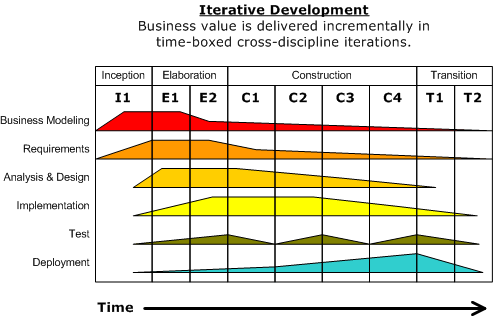
\includegraphics[scale=0.7]{./Figures/RUP.png}
	\caption[Rational Unified Process]
	{Iterative development cycle of Rational Unified Process.}
	\label{fig:RUP}
\end{figure}

Now we have acknowledged some development processes that are commonly used in
the industry for creating software applications. Model Driven Engineering is a
software development methodology which focuses on creating and exploiting
models. And by using these models,  MDE aims at improving productivity and
quality in software development. This is achieved by not only to use models as
documentation, but instead to use models as the major artifact in a software
development cycle. The idea is to use models at different levels of abstraction
and apply model transformations to automate the implementation on these
models.
This will raise the level of abstraction in program and problem specification.
We can divide these models into two main model classes, namely development
models and runtime models\cite{France2007}. Development models is used as an
abstraction above code level. These models could represent software
requirements, work flow, architecture and software implementation. These
development models are most typically used in software development process that
we described above as a supplement in developing an application. Runtime models

\subsection{Model Driven Architecture}

\begin{figure}[H]
	\centering
	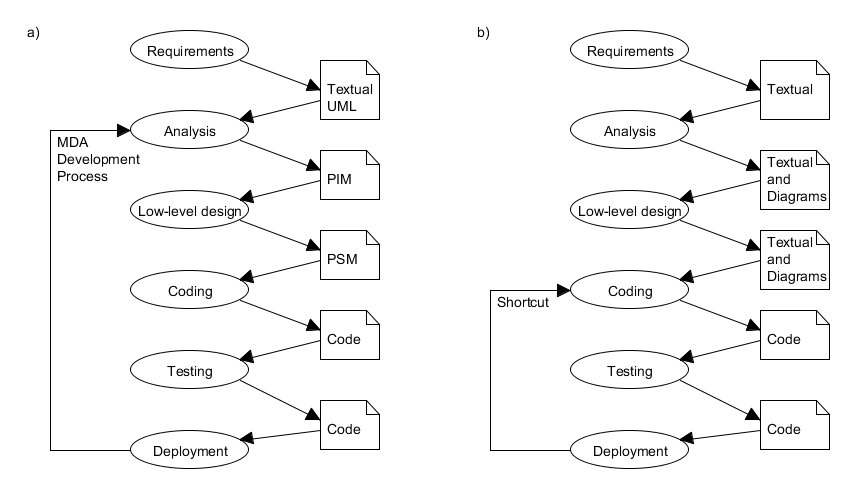
\includegraphics[scale=0.5]{./Figures/MDA.png}
	\caption[Software Development with MDA]
	{a) Model-Driven-Architecture and b) Traditional development process}
	\label{fig:MDA}
\end{figure}



%-----------------------------------
%	SUBSECTION 1
%-----------------------------------
\section{Metamodelling}

Metamodelling plays a vital role in model driven engineering (MDE) to describe a
modelling language. A metamodel defines the abstract syntax and provides a
description of a modelling language. Another popular definition for
metamodeling is that it is a ``model of models". This definition is both
unhelpful and incorrect according to Steve Cook and Stuart Kent in their
paper\cite{Cook2008}. They think that a better definition for a metamodel is
that ``it is a model of the concepts expressed by a modelling language.'' A
metamodel is basically a model that is specified by a metamodelling language.
The exact definition of a metamodel is highly debated amongst MDE
researchers\cite{Rutle}. When creating instance of these metamodels we can
specify a Domain Specific Modelling Language (DSML) from the concrete syntax of
a metamodel.

\begin{figure}[H]
	\centering
	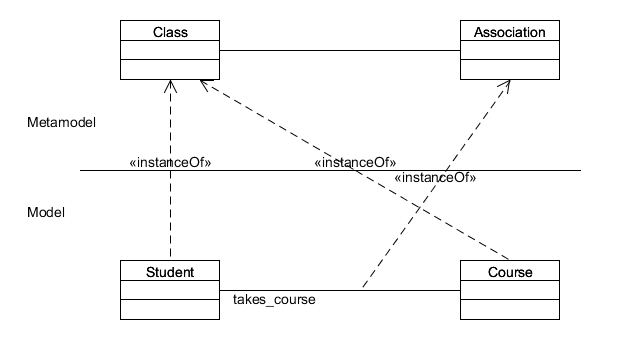
\includegraphics[scale=0.6]{./Figures/SimpleMetamodel.png}
	\caption[Example of a model and metamodel]
	{A simple example of a model and its metamodel.}
	\label{fig:SimpleMetamodel}
\end{figure}

Figure~\ref{fig:SimpleMetamodel} shows a simple example of a instance model and
its corresponding metamodel. This model has two nodes, Student and Course, and
bidirectional an association, take course and has students, that connect these
two nodes. The model is specified by some modelling language, namely
UML\cite{UML}, that conforms to a metamodel. This metamodel consists of two
metaclasses Class and Association and one bidirectional association between
them. Both Student and Course are an instance of the metaclass Class, while the
association between Student and Course are instance of the metaclass
Association. We use metamodels when we want to define a modelling language.

\begin{figure}[H]
	\centering
	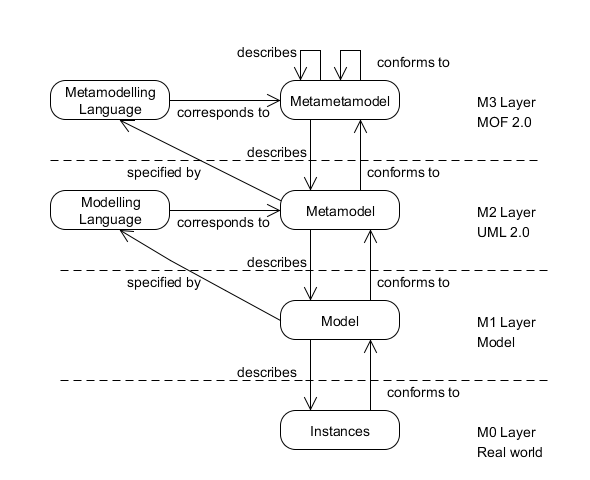
\includegraphics[scale=0.6]{./Figures/MOFLayers.png}
	\caption[Meta Object Facility]
	{Example of Meta Object Facility and its four layers.}
	\label{fig:MOFLayers}
\end{figure}



%-----------------------------------
%	SUBSECTION 2
%-----------------------------------

\subsection{MOF}


%----------------------------------------------------------------------------------------
%	SECTION 2
%----------------------------------------------------------------------------------------

\section{Constraints}

\subsection{Structural Constraints}

\subsection{Attached Constraints}

\section{Workbenches}

\subsection{Eclipse Platform}

\subsubsection{EMF}

\section{DPF}

\section{DPF Editor}
 
